\chapter{Methods}\label{chap:methods}
\begin{chapabstract}

In this chapter, I describe procedures of our study from making a subsample of HRS galaxies to calculating the radio SFR\@.
Section~\ref{sec:crossmatching} and~\ref{sec:reducegalaxysamples} show how to select samples from two catalogs introduced in the previous section for $\qn$ analysis henceforth.
Section~\ref{sec:calculatingq} gives the definition of $\qn$ and the way to apply it for our samples.
Section~\ref{sec:tirluminosity} describes the method to estimate total IR luminosity from several IR bands' observations.
Section~\ref{sec:fittingtoq} shows how to find the frequency dependence of $\qn$ by the fitting.
Section~\ref{sec:calculatingsfr} describes how to calculate SFR from the low-frequency radio emission.

\end{chapabstract}

\section{Cross Matching}\label{sec:crossmatching}
Although HRS galaxies have been studied in multi-wavelength observations, their spectral energy distribution around $100\MHz$ is not well-understood \citep{Ciesla2014}, where the contribution from synchrotron radiation is much more significant than from free-free emission \citep{Condon1992a}.
Here, I provide a procedure to cross-matching with two different catalogs I have mentioned in the previous chapter.
Cross-matching is the method widely used in astronomy to obtain additional information from other surveys or catalogs by matching coordinates of each galaxy or blob source within a specific error (e.g., $\sim 1.0\,\mr{arcsec}$).
For executing this method for the HRS and the GLEAM survey catalog, we use Tool for OPerations on Catalogues And Tables (TOPCAT\@; \citealt{Taylor2009}).
TOPCAT is a popular and useful tool for dealing with catalogs and tables, and it allows us to do the cross-matching easily, even more than two catalogs.

Initially, we assume a $10\,\mr{arcsec}$ error radius for the cross-matching since it is equivalent to the value of $95\%$ error for the astrometry in the GLEAM survey (Section 4.5.5 in \citealt{Hurley-Walker2017a}).
This matching results in a total of 18 galaxies, which are identified to have a radio counterpart.
To assess the matching, we compare a separation of counterparts from the center of galaxies with coordinate uncertainties in the GLEAM catalog.
For these galaxies, we find 15 of them have a separation within a 95\% error radius, and others do not.
Although three of them have a more significant separation compared to the error radius, we conclude that the matching for all 18 galaxies is correct by the checking of galaxy images (Appendix~\ref{chap:galaxyimages}).
In our study, we regard a radio blob as a counterpart if the brightest part of each blob where the inside of the contour nearest to the center, is surrounded by the D25 radius (the isophotal optical size at $25\,\mr{mag}\arcs^{-2}$; \citealt{Boselli2010}).

Next, we extend the error radius up to $120\arcs$, which is corresponding to the angular resolution of the GLEAM survey at $200\MHz$.
This operation is executed because the radio sources are blurred due to the angular resolution of the GLEAM survey, and the location of them might be shifted.
We know $120\arcs$ error radius is quite big for the matching, but this trial gives us the inspiration for the cross-matching with blurred radio sources in the future study.
The cross-matching with the error of $120\arcs$ suggests that there are 25 new galaxies have a potential counterpart.
To assess these matching, we look at galaxy images one by one.
With the same condition mentioned above, we identify 21 matches for these galaxies.

Although we have identified a total of 39 matches in the same way, there are six suspicious matches because of interacting counterparts (HRS4, 216, 244, 284) and quite large separations (HRS200, 295) (Figure~\ref{fig:galaxyimages_suspicious}).
For these galaxies, we flag them as suspicious matches, and we do not use them for further analysis.
The distribution of separations for galaxies showed in Figure~\ref{fig:separation}.

\begin{figure}[htbp]
	\centering
	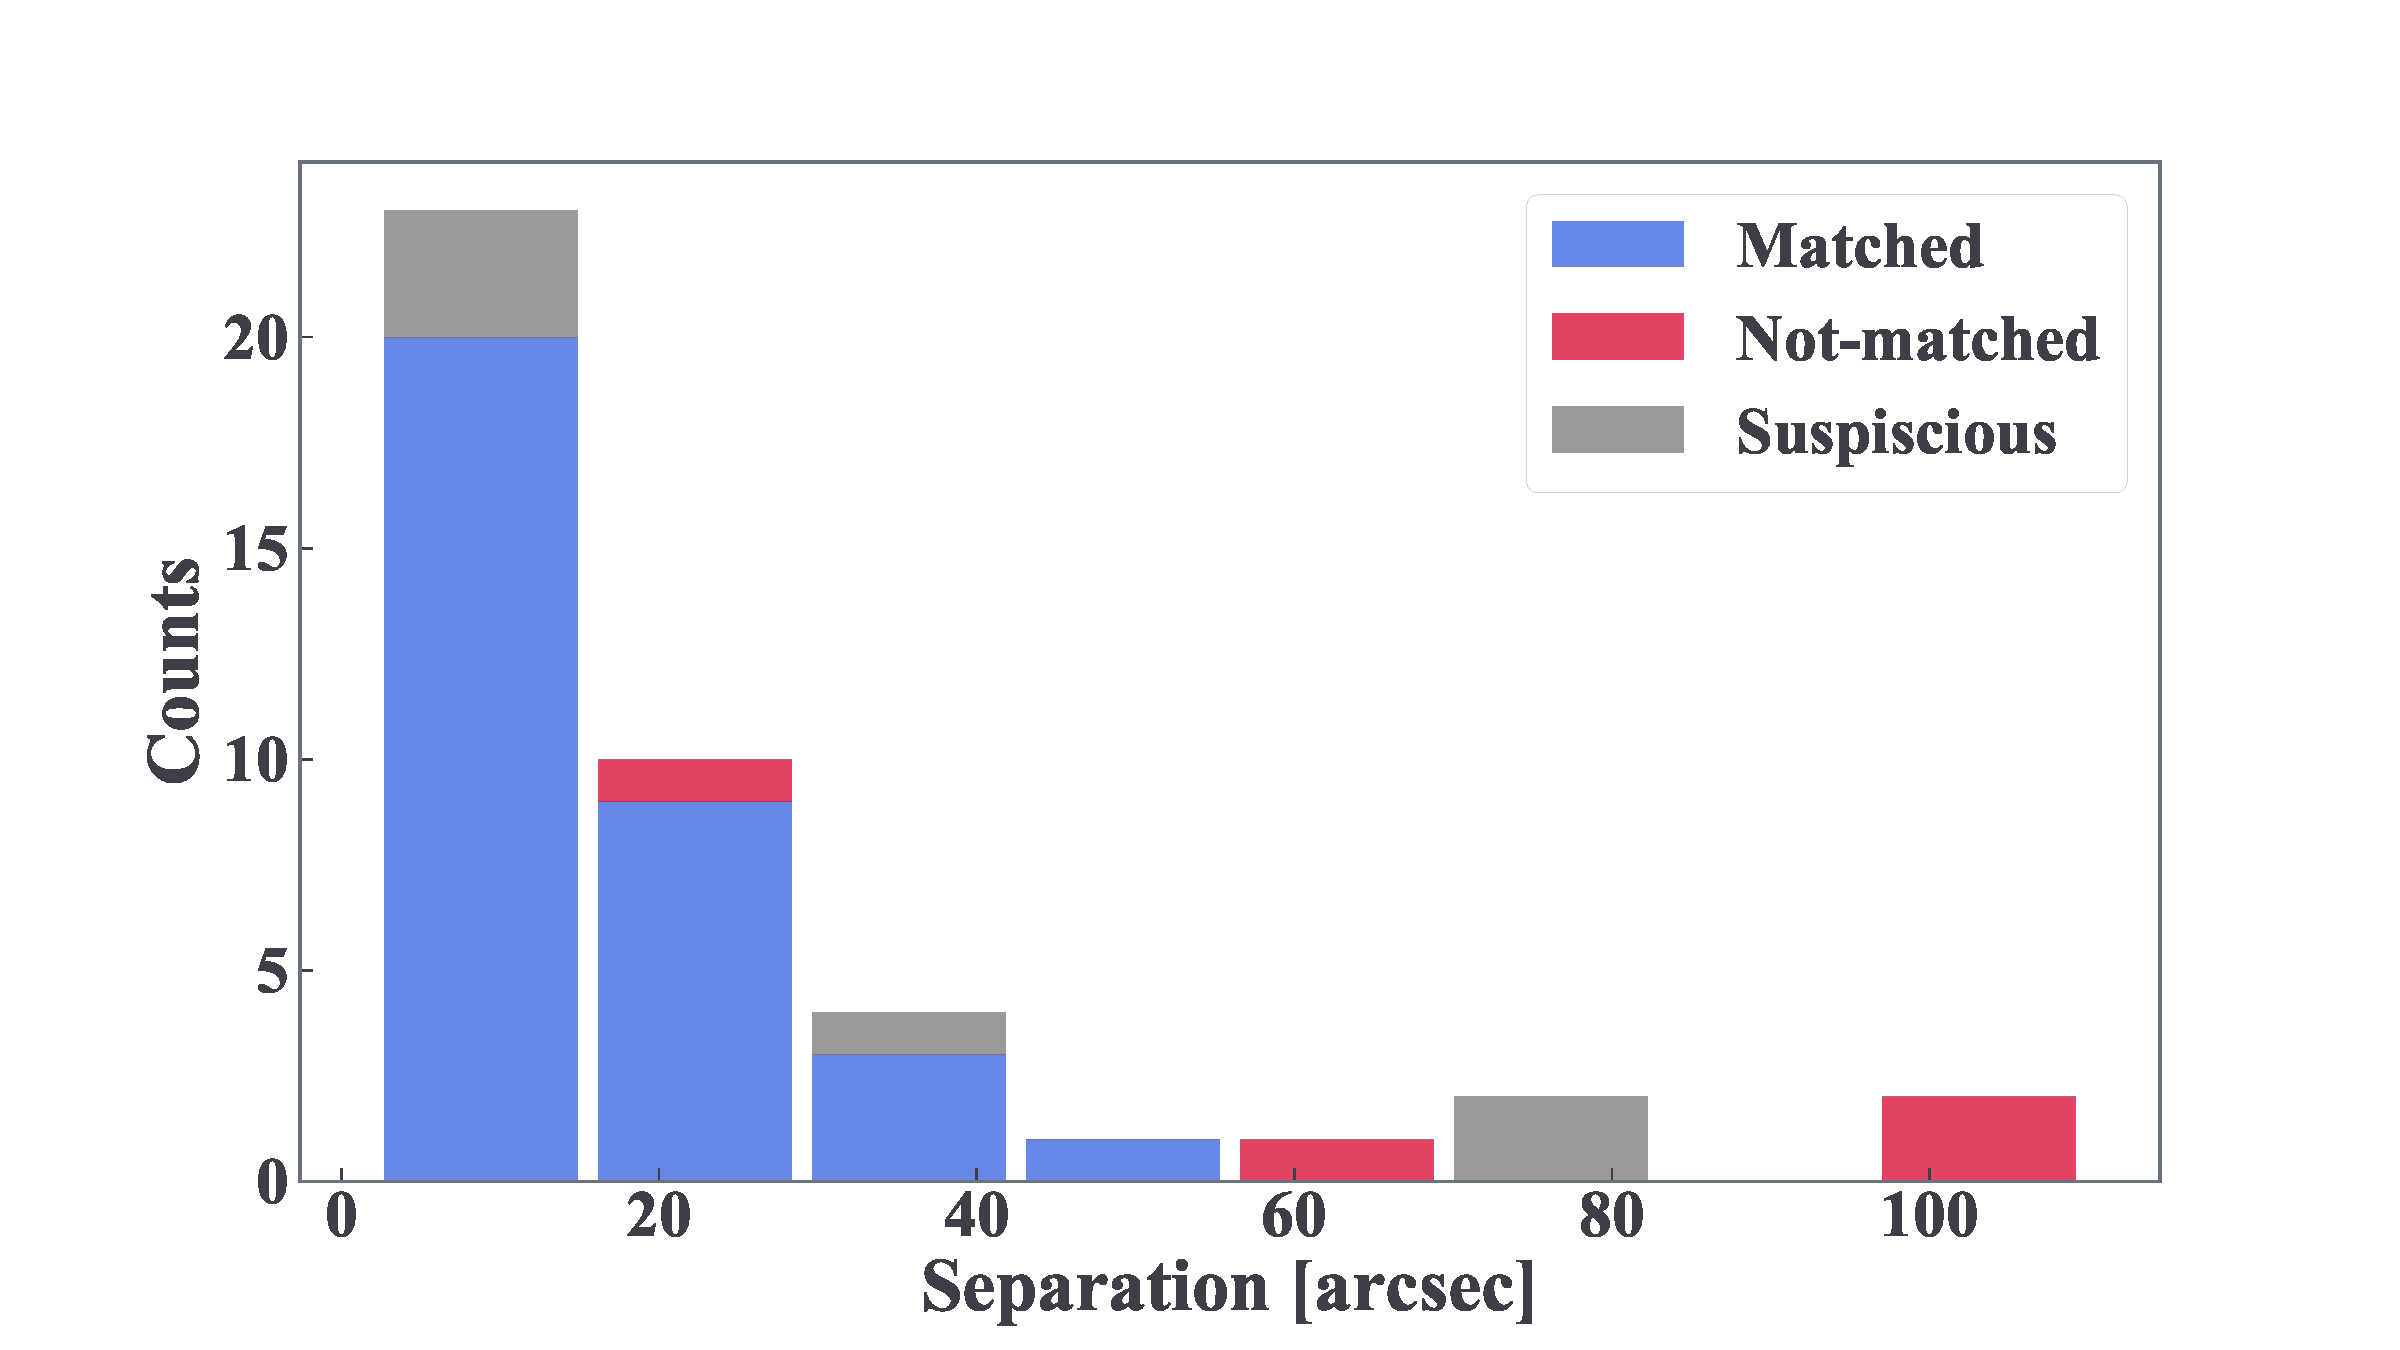
\includegraphics[width=.8\linewidth]{Chapter_4/Figures/Method_separation.pdf}
    \caption[Separation from the cross-matching]{\label{fig:separation}
        This figure shows the distribution of separations.
        Here we put 43 galaxies and color sorted based on the result.
        The blue bar shows galaxies identified to have a radio counterpart, red one does galaxies determined not to have a counterpart, and gray for the suspicious galaxies.
        Most of the matched samples are distributed within a $40\,\mr{arcsec}$ error radius.
    }
\end{figure}

We put all galaxy images cross-matched within $120\,\mr{arcsec}$ in Appendix~\ref{chap:galaxyimages}.



\section{Select galaxy samples for a reliable analysis}\label{sec:reducegalaxysamples}

In this section, we show some steps for selecting galaxies to do a reliable analysis.
Since we focus on the relation of galaxy radio emission with star formation activities, we should clarify the radio source and be sure that they are not originally from other sources rather than the star formation.
The radio emission arisen from the star formation activities should be proportional to the SFR in a galaxy \citep{Condon1992a, Murphy2011}.
However, elliptical galaxies have a stronger radio emission against their star formation.
In this case their radio emission would be emitted by not star-forming sources.
These radio sources are considered as Active Galactic Nuclei (AGN), which emits strong radio emission due to the baryon accretion into the supermassive black hole at the center of galaxies irrelevant to the star formation \citep[e.g.,][]{Urry1995, Padovani2017}.
According to the morphology of galaxies \citep{Cortese2012}, we identify four elliptical galaxies (HRS49, 138, 178, 241) and they are not used for further calculation and discussion.
%With these operations, we finally find that there are 37 HRS galaxies are available for further analysis.

After this galaxy selection, we obtain 29 galaxies with a reliable radio counterpart arisen from the star formation activity.

As a next step, we evaluate the signal to noise ratio (SNR) of radio emission at each MWA band.
For reducing the uncertainty caused by observational errors, we assess the peak flux at each narrow band by comparing it to the local noise level and adopt flux values whose SNR is higher than five.
This analysis results in a total of 11 galaxies have no radio fluxes whose SNR is higher than the criterion.
The reason why these radio sources are detected although they do not have any fluxes with higher SNR, is \citet{Hurley-Walker2017a} determine the detection based on the SNR in the stacking images ($170\mbox{--}231\MHz$).
%\vspace{0.3cm}\\

Finally, after the cross-matching and these procedures, we confirm 18 HRS galaxies are the samples available for further analysis.
The overview of 18 samples is tabled in Appendix~\ref{chap:galaxysamples}.



\section{Calculating the $\qn$ parameter}\label{sec:calculatingq}
In this section, I introduce the method to calculate the $\qn$ parameter, which shows the ratio between integrated IR and radio luminosities in a galaxy.
The definition of this parameter here is given on the following equation \citep[e.g.,][]{Helou1985, Bell2003, CalistroRivera2017a}:

\begin{equation}\label{eq:q_def}
    \qn \equiv \log\brp{\frac{L\msb{8\mbox{--}1000\,\mu m}\ /\ 3.75 \times 10^{12}}{{\rm erg\,s^{-1}\,Hz^{-1}}}} - \log\brp{\frac{L_{\mr{Radio},\,\nu}}{{\rm erg\,s^{-1}\,Hz^{-1}}}}
\end{equation}
where $L\msb{8\mbox{--}1000\,\mu m}$ is the total rest-frame infrared luminosity among $8 \mbox{--} 1000\,\mr{\mu m}$ and $3.75\times10^{12}\,\mr{Hz}$ is equivalent to the frequency of $80\,\mr{\mu m}$ for correcting the dimension.

Although \citet{Ciesla2014} have already derived the total IR luminosity for most HRS galaxies using the SED fitting, one of our galaxy samples (HRS163) does not have the value because of the lack of the reliable mid-IR flux from {\it Spitzer\/} telescope.
For consistency, we adopt the total IR luminosity calculated from the same method for all galaxy samples.
%To calculate the total IR luminosity, we refer to \citet{Galametz2013}, which derive the calibration relation between combining monochromatic IR luminosities and the total IR luminosity.
To calculate the total IR luminosity, we refer to \citet{Galametz2013}, which derives the calibration relation of the total IR luminosity with monochromatic IR luminosities.
We show the procedure to calculate total IR luminosity in the next section.



\section{Total IR luminosity}\label{sec:tirluminosity}
In this section, I present how to calculate the total IR luminosity in this study.
For the method of calculating total IR luminosity, we refer to \citet{Galametz2013}, which shows the empirical relations to estimate total IR from {\it Spitzer\/} ($24, 70\micron$) and {\it Herschel\/} bands ($100, 160, 250\micron$).
HRS galaxies have flux data from the Multiband Imaging Photometry for {\it Spitzer\/} (MIPS;~\citealt{Rieke2004, Bendo2012}), the {\it Herschel\/}/PACS ($100,\,160\micron$; \citealt{Cortese2014c}) and the {\it Herschel\/}/SPIRE ($250\micron$; \citealt{Ciesla2012a}).

\citet{Galametz2013} derived the calibration equation below:

\begin{equation}\label{eq:galametz}
    L\msb{3\mbox{--}1100\mr{\mu m}} = \sum c_i \nu L_{\nu}\left(i\right)
\end{equation}
where $L\msb{3\mbox{--}1100\,\mu m}$ is the total IR luminosity in the frequency range from 3 to 1100 $\mr{\mu m}$, $c_i$ is the coefficients at $i = 24,\,70,\,100,\,160,\,250\,\mathrm{\mu m}$, and $L_{\nu}$ is the luminosity at the frequency $\nu$ corresponds to a specific wavelength $i$.
For deriving $L_{\nu}$, we calculate it from fluxes and the distance to each galaxy.
We refer to \citet{Cortese2012} for obtaining galaxy distances.

\citet{Galametz2013} derived the conversion equation with at least two bands.
Therefore, we can estimate total IR luminosities even if galaxies are lack of a few fluxes.
Since several calculations in the following sections require the total IR luminosity among $8 \mbox{--} 1000\micron$ ($L\msb{8\mbox{--}1000\micron}$), we recalibrate this luminosity by multiplying the constant value (0.88) in \citet{Takeuchi2005}.

The total IR luminosity calculated here is consistent with that of \citet{Ciesla2014} within factor 2 (Figure~\ref{fig:tircomparison}).

\begin{figure}[htbp]
	\centering
	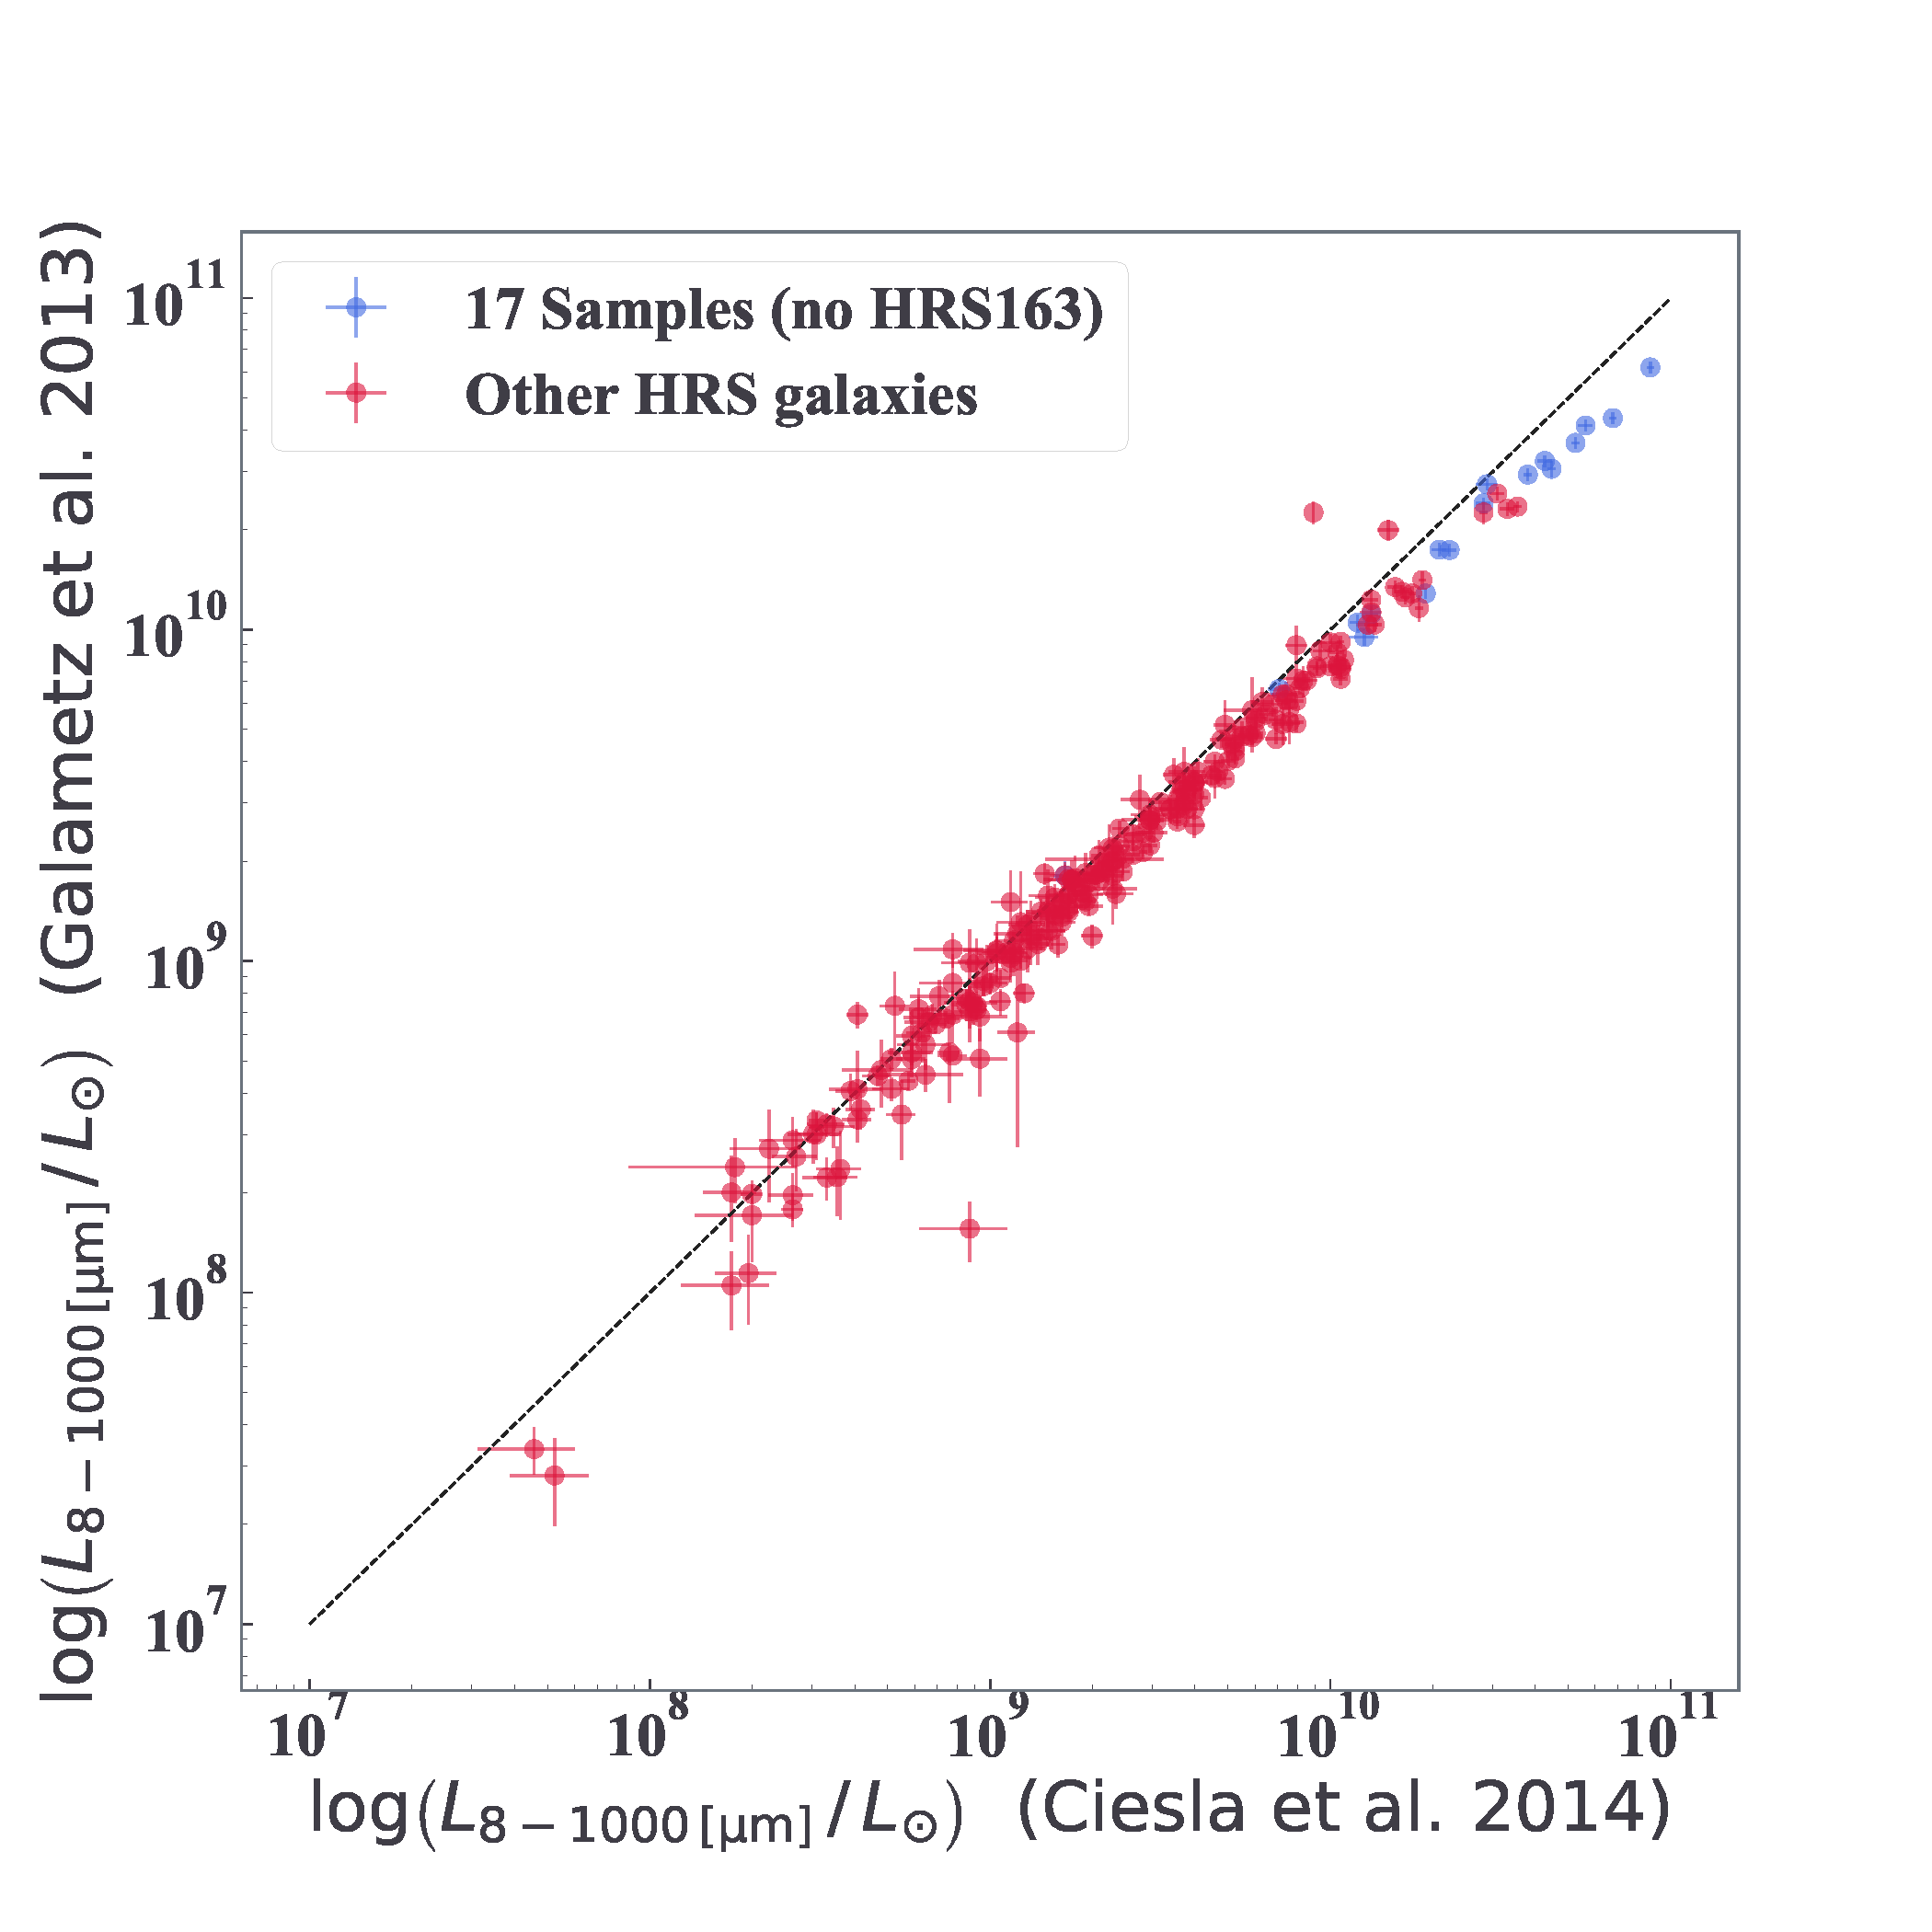
\includegraphics[width=.7\linewidth]{Chapter_4/Figures/Method_TIRcomparison.pdf}
    \caption[The comparison of total IR luminosities]{\label{fig:tircomparison}
        This figure shows the comparison of total IR luminosity at $8\mbox{--}1000\micron$ from different methods.
        Here, we show all HRS galaxies which have both luminosities.
        Blue plots show galaxy samples selected in Section~\ref{sec:crossmatching} and~\ref{sec:reducegalaxysamples}, and red ones show other HRS galaxies.
        The difference of both luminosities is less than factor 2.
    }
\end{figure}

Hereafter, we use $L_{8\mbox{--}1000\mathrm{\mu m}}$ obtained here to calculate the $\qn$ parameter and SFRs.



\section{Fitting to $\qn$ parameters}\label{sec:fittingtoq}
Here, we show how to do the fitting to $\qn$.
%If I add the chapter 2, delete after , which emitted from~~~
At low frequencies around $100\MHz$, the synchrotron radiation can be dominant, which emitted from high energy electrons accelerated by the supernova remnant.
In this paper, we assume radio emission has a single power-law on the frequency and adopt the following equation:

\begin{equation}\label{eq:q_fitting}
    q_{\nu} = -\gamma\log{\nu} + \beta
\end{equation}
where $q_{\nu}$ is defined by Equation~\ref{eq:q_def} at $\nu\MHz$, $\gamma$ is the power-law index showing the frequency dependence of $\qn$, and $\beta$ is the second fitting parameter.

In this study, we execute two types of fitting:

\begin{enumerate}
    \item Fitting to only MWA frequencies ($72\mbox{--}231\MHz$)
    \item Fitting to $1500\MHz$ besides MWA frequencies
\end{enumerate}

The flux data at $1500\MHz$ is obtained from \citet{Boselli2015}, and here we use only high-quality flux data (flag = 1 in \citealt{Boselli2015}).
These two types of fitting might allow us to judge the correctness of a single power-law assumption.
These fitting results are summarized in Section~\ref{sec:GammaDistribution}.



\section{Calculating the SFR}\label{sec:calculatingsfr}
In this section, I describe how to derive SFR from low-frequency radio emissions.\\
Here, we estimate the radio SFR, combining Equation~\ref{eq:q_def} with the following equations:

\begin{align}
    \mr{SFR}\msb{IR} &= 3.88 \times 10^{-44}\brp{\frac{L\msb{8\mbox{--}1000\,\mu m}}{\mr{erg}\,s^{-1}}}\label{eq:sfrir}\\
    q_{\nu\,\mr{MHz}} &= \q{1500\MHz} + \log{\brp{\frac{\nu\,\mr{MHz}}{1500\,\mr{MHz}}}}^{\gamma}\label{eq:q_nuto1500}
\end{align}

Equation~\ref{eq:sfrir} calculates SFR from the total IR emission in \citet{Murphy2011}, and Equation~\ref{eq:q_nuto1500} shows the difference of the $\qn$ between a certain wavelength $\nu$ and $1500\MHz$.

Substituting equation~\ref{eq:q_def} and~\ref{eq:q_nuto1500} into equation~\ref{eq:sfrir} yields the following equation to estimate SFR from the radio emission at $\nu\MHz$:

\begin{equation}\label{eq:sfrfromradio}
    \mr{SFR}_{\mr{Radio},\,\nu} = 1.46\times10^{-31}\times 10^{q\msb{1500\MHz}} {\brp{\frac{\nu\,\MHz}{1500\MHz}}}^{-\gamma} \times L_{\mr{Radio},\,\nu}
\end{equation}

In Section~\ref{sec:sfrfromlowradio}, I show the results of calculating SFR from the low-frequency radio using this equation and comparing it with the SFR from other indicators.



%\bibliographystyle{mnras}
%%\bibliography{example} % if your bibtex file is called example.bib
%\bibliography{masterthesis}
